%\documentclass[preprint,12pt]{elsarticle}

%% Use the options 1p,twocolumn; 3p; 3p,twocolumn; 5p; or 5p,twocolumn
%% for a journal layout:
%%  \documentclass[final,1p,times]{elsarticle}
%% \documentclass[final,1p,times,twocolumn]{elsarticle}
%% \documentclass[final,3p,times]{elsarticle}
%% \documentclass[final,3p,times,twocolumn]{elsarticle}
%\documentclass[final,5p,times]{elsarticle}
\documentclass[final,5p,times,twocolumn]{elsarticle}

%% if you use PostScript figures in your article
%% use the graphics package for simple commands
%% \usepackage{graphics}
%% or use the graphicx package for more complicated commands
%% \usepackage{graphicx}
%% or use the epsfig package if you prefer to use the old commands
%% \usepackage{epsfig}

%% The amssymb package provides various useful mathematical symbols
\usepackage{amssymb}

\usepackage{makeidx}  % allows for indexgeneration
\usepackage{algorithm,algpseudocode}
\usepackage{graphicx}
\usepackage{float}
\usepackage{subcaption}
\captionsetup{compatibility=false}
\usepackage{wrapfig}
\usepackage{array}
\usepackage{multicol}

%\usepackage{cite}
% The amsthm package provides extended theorem environments
%% \usepackage{amsthm}


\journal{Future Generation of Computer Systems}

\begin{document}

\begin{frontmatter}


\title{Scientific Workflow Analysis with Quantitative and Structural Metrics}


\author[isi]{Weiwei Chen\corref{cor1}}
\ead{weiweich@acm.org}

\author[isi]{Rafael Ferreira da Silva}
\ead{rafsilva@isi.edu}

\author[isi]{Ewa Deelman}
\ead{deelman@isi.edu}


\author[man]{Rizos Sakellariou}
\ead{rizos@cs.man.ac.uk}

\cortext[cor1]{Corresponding address: USC Information Sciences Institute, 4676 Admiralty Way Ste 1001, Marina del Rey, CA, USA, 90292, Tel: +1 310 448-8408}


\address[isi]{University of Southern California, Information Sciences Institute, Marina del Rey, CA, USA}
\address[man]{University of Manchester, School of Computer Science, Manchester, U.K.}


\begin{abstract}
As scientific workflows grow in complexity and importance, the designers of scientific workflows need a deeper and broader understanding of the characteristics and features of workflows and how they behave in order to improve the overall performance. 
This paper provides a quantitative, structural, and overhead aware analysis of workflows of diverse scientific applications, including astronomy, bioinformatics, earthquake science, and gravitational-wave physics. The workflow analysis is based on novel workflow structural metrics that provide substantial information about the characteristics of workflow structures and concretely show how they influence the overall performance. 
%This information includes density, overlap, and sensitivity etc.. 
This paper further applies these metrics to three popular workflow research scenarios including workflow profiling, task clustering, and overhead aware task scheduling. Trace based analysis and simulations show their strong capabilities in revealing hidden information and driving improvements on workflow performance. 

\end{abstract}

\begin{keyword}
Scientific workflows \sep Performance analysis \sep Scheduling \sep Workflow Simulation
\end{keyword}

\end{frontmatter}


\section{Introduction}
\label{intro}
Many computational scientists develop and use large-scale, loosely-coupled applications that are often structured as scientific workflows. Although the majority of the tasks within these applications are often relatively short running (from a few seconds to a few minutes), in aggregate they represent a significant amount of computation and data~\cite{daSilva:2013:TFO:2534248.2534254,Juve2013}. When executing these applications in a multi-machine{, }distributed environment, such as the Grid or the Cloud, significant system overheads may exist and may slowdown the application {execution}~\cite{Chen2011}. To reduce the impact of such overheads, task clustering techniques~\cite{Muthuvelu:2005:DJG:1082290.1082297,4493929,Muthuvelu2010,Muthuvelu2013170,keat-2006,ang-2009,Liu2009,Singh:2008:WTC:1341811.1341822,Ferreira-granularity-2013} have been developed to group \emph{fine-grained} tasks into \emph{coarse-grained} tasks so that the number of computational activities is reduced and {so that }their computational granularity is increased{.  This reduced }the (mostly scheduling related) system overheads.
However, there are several challenges that have not yet been addressed.

A scientific workflow is typically represented as a directed acyclic graph (DAG). {The nodes represent computations and the edges describe data and control dependencies between them. }Tasks within a level (or depth within a workflow DAG) may have different runtimes. {Proposed task clustering techniques that merge  }tasks within a level without considering the runtime variance may cause load imbalance, i.e., some clustered jobs may be composed of short running tasks while others of long running tasks. This imbalance delays the release of tasks from the next level of the workflow, penalizing the workflow execution with an overhead produced by the use of inappropriate task clustering strategies~\cite{Chen2013}.
A common technique to handle load imbalance is overdecomposition~\cite{Lifflander}.
This method decomposes computational work into \emph{medium-grained} balanced tasks. Each task is coarse-grained enough to enable efficient execution and reduce scheduling overheads, while being fine-grained enough to expose significantly higher application-level parallelism than what is offered by the hardware. 

Data dependencies between workflow tasks play an important role when clustering tasks within a level. A data dependency means that there is a data transfer between two tasks (output data for one and input data for the other). Grouping tasks without considering these dependencies may lead to data locality problems{, }where output data produced by parent tasks are poorly distributed. As a result, data transfer times and failure probabilities increase.
Therefore, we claim that data dependencies of subsequent tasks should be considered.

We generalize these two challenges (Runtime Imbalance and Dependency Imbalance) to the general task clustering load balance problem. We introduce a series of balancing methods to address these challenges. However, there is a tradeoff between runtime and data dependency balancing. For instance, balancing runtime may aggravate the Dependency Imbalance problem, and vice versa. Therefore, we propose a series of quantitative metrics that reflect the internal structure (in terms of task runtimes and dependencies) of the workflow and use them as a criterion to select and balance {the } solutions.

In particular, we provide a novel approach to capture {the imbalance } metrics. Traditionally, there are two approaches to improve the performance of task clustering. The first one is a top-down approach \cite{6217508} that represents the clustering problem as a global optimization problem and aims to minimize the overall workflow execution time. However, the complexity of solving such an optimization problem does not scale well since most solutions are based on genetic algorithms. The second one is a bottom-up approach~\cite{Muthuvelu:2005:DJG:1082290.1082297,Liu2009} that only examines free tasks to be merged and optimizes the clustering results locally. In contrast, our work extends these approaches to consider the neighboring tasks including siblings, parents, and children{, } because such a family of tasks has strong connections between them. 

The quantitative metrics and balancing methods were introduced and evaluated in~\cite{6683907} on {five }workflows. In this {paper}, we extend this previous work by studying:

\begin{itemize}[noitemsep,nolistsep]
	\item the performance gain of using our balancing methods over a baseline execution on a larger set of workflows;
	\item the performance gain over two additional task clustering methods described in the literature~\cite{ang-2009,Liu2009};
	\item the performance impact of the variation of the average data size and number of resources;
	\item the performance impact of combining our balancing methods with vertical clustering.
\end{itemize}

The rest of {the paper } is organized as follows. Section~\ref{sec:related-work} gives an overview of the related work. Section~\ref{sec:model} presents our workflow and execution environment models. Section~\ref{sec:imbalance} details our heuristics and algorithms for balancing. Section~\ref{sec:experiments} reports experiments and results, and the {paper } closes with a discussion and conclusions.

% Section
\section{Related Work}
\label{sec:related-work}

{System }overhead analysis~\cite{Ostberg2011, Prodan2008} is a topic of great interest in the {distributed computing } community. Stratan et al.~\cite{Stratan2008} evaluate in a real-world environment Grid workflow engines including DAGMan/Condor and Karajan/Globus. Their methodology focuses on five system characteristics: overhead, raw performance, stability, scalability, and reliability. They {point } out that {resource consumption in head nodes }should not be {ignored } and {that } the main bottleneck in a busy system is often the head node. Prodan et al.~\cite{Prodan2008} offered a complete Grid workflow overhead classification and a systematic measurement of overheads. In Chen et al.~\cite{Chen2011}, we extended~\cite{Prodan2008} by providing a measurement of major overheads imposed by workflow management systems and execution environments and analyzed how existing optimization techniques improve {the workflow }runtime by reducing or overlapping overheads. The prevalent existence of system overheads is an important reason why task clustering provides significant performance improvement for workflow-based applications. In this chapter, we aim to further improve the performance of task clustering under imbalanced load. 

The low performance of \emph{fine-grained} tasks is a common problem in widely distributed platforms where the scheduling overhead and queuing times at resources are high, such as Grid and Cloud systems. Several works have addressed the control of task granularity of bags of tasks. For instance, Muthuvelu et al.~\cite{Muthuvelu:2005:DJG:1082290.1082297} proposed a clustering algorithm that groups bags of tasks based on their runtime---tasks are grouped up to the resource capacity. Later, they extended their work~\cite{4493929} to determine task granularity based on task file size, CPU time, and resource constraints. Recently, they proposed an online scheduling algorithm~\cite{Muthuvelu2010,Muthuvelu2013170} that groups tasks based on resource network utilization, user's budget, and application deadline. Ng et al.~\cite{keat-2006} and Ang et al.~\cite{ang-2009} introduced bandwidth in the scheduling framework to enhance the performance of task scheduling. Longer tasks are assigned to resources with better bandwidth. Liu and Liao~\cite{Liu2009} proposed an adaptive fine-grained job scheduling algorithm to group fine-grained tasks according to processing capacity and bandwidth of the current available resources. Although these techniques significantly reduce the impact of scheduling and queuing time overhead, they {do } not consider data dependencies.

Task granularity control has also been addressed in scientific workflows. For instance, Singh et al.~\cite{Singh:2008:WTC:1341811.1341822} proposed level- and label-based clustering. In level-based clustering, tasks at the same level {of the workflow }can be clustered together. The number of clusters or tasks per cluster are specified by the user. In the label-based clustering {method}, the user labels tasks that should be clustered together. Although their work considers data dependencies between workflow levels, it is done manually by the users, which is prone to errors {and it is not scalable}. Recently, Ferreira da Silva et al.~\cite{Ferreira-granularity-2013,FerreiradaSilva-CCPE-2014} proposed task grouping and ungrouping algorithms to control workflow task granularity in a non-clairvoyant and online context, where none or few characteristics about the application or resources are known in advance. Their work significantly reduced scheduling and queuing time overheads, but did not consider data dependencies.

A plethora of balanced scheduling algorithms have been developed in the networking and operating system domains. Many of these schedulers have been extended to the hierarchical setting. Lifflander et al.~\cite{Lifflander} proposed to use work stealing and a hierarchical persistence-based rebalancing algorithm to address the imbalance problem in scheduling. Zheng et al.~\cite{Zheng} presented an automatic hierarchical load balancing method that overcomes the scalability challenges of centralized schemes and poor solutions of traditional distributed schemes. There are other scheduling algorithms~\cite{rizos2008} that indirectly achieve load balancing of workflows through makespan minimization. However, the benefit that can be achieved through traditional scheduling optimization is limited by its complexity. The performance gain of task clustering is primarily determined by the ratio between system overheads and task runtime, which is more substantial in modern distributed systems such as Clouds and Grids. 

Workflow patterns~\cite{Yu2005a, Juve2013, Liu2008} are used to capture and abstract the common structure within a workflow and they give insights on designing new workflows and optimization methods. Yu and Buyya~\cite{Yu2005a} proposed a taxonomy that characterizes and classifies various approaches for building and executing workflows on Grids. They also provided a survey of several representative Grid workflow systems developed by various projects world-wide to demonstrate the comprehensiveness of the taxonomy. Juve et al.~\cite{Juve2013} provided a characterization of workflow from six scientific applications and obtained task-level performance metrics (I/O, CPU, and memory consumption). They also presented an execution profile for each workflow running at a typical scale and managed by the Pegasus workflow management system~\cite{Deelman2004, Deelman:2005:PFM:1239649.1239653, deelman2014pegasus}. Liu et al.~\cite{Liu2008} proposed a novel pattern based time-series forecasting strategy which utilizes a periodical sampling plan to build representative duration series. We illustrate the relationship between the workflow patterns (asymmetric or symmetric workflows) and the performance of our balancing algorithms. 

Some work in the literature has further attempted to define and model workflow characteristics with quantitative metrics. In~\cite{Ali2004}, the authors proposed a robustness metric for resource allocation in parallel and distributed systems and accordingly customized the definition of robustness. Tolosana et al.~\cite{Tolosana2011} defined a metric called Quality of Resilience to assess how resilient workflow enactment is likely to be in the presence of failures. Ma et al. ~\cite{Ma:2014:GDB:2560969.2561388} proposed a graph distance based metric for measuring the similarity between data oriented workflows with variable time constraints, where a formal structure called time dependency graph (TDG) is proposed and further used as representation model of workflows. Similarity comparison between two workflows can be reduced to computing the similarity between TDGs. In this work, we develop quantitative metrics to measure the severity of the imbalance problem in task clustering and then use the results to guide the selection of different task clustering methods.



\section{Model and Design}
\label{sec:model}


\begin{figure}[htb]
	\centering
	\includegraphics[width=0.7\linewidth]{figures/model/odag.pdf}
	\captionof{figure}{Extending DAG to o-DAG.}
	\label{fig:model_odag}
	\vspace{-10pt}
\end{figure}
A workflow is modeled as a Directed Acyclic Graph (DAG) as shown in Fig.~\ref{fig:model_odag} (Left). Each node in the DAG often represents a workflow job ($j$), and the edges represent dependencies between the jobs that constrain the order in which the jobs are executed. Dependencies typically represent data-flow dependencies in the application, where the output files produced by one job are used as inputs of another job. Each job is a single execution unit and it may contains one or multiple tasks, which is a program and a set of parameters that need to be executed. Fig.~\ref{fig:model_odag} (left) shows an illustration of a DAG composed by four jobs. This model fits several workflow management systems such as Pegasus~\cite{Deelman2005}, Askalon~\cite{Fahringer2005}, and Taverna~\cite{Oinn:2006:TLC:1148437.1148448}.

%Change it with job wrapper
Fig.~\ref{fig:model_system} shows a typical workflow execution environment. The submit host prepares a workflow for execution (clustering, mapping, etc.), and worker nodes, at an execution site, execute jobs individually. The main components are introduced below:

\begin{figure}[htb]
\centering
  \includegraphics[width=0.95\linewidth]{figures/model/execution.pdf}
  \caption{A workflow system model.}
  \label{fig:model_system}
  \vspace{-10pt}
\end{figure}

\paragraph{Workflow Mapper} generates an executable workflow based on an abstract workflow provided by the user or workflow composition system. It also restructures the workflow to optimize performance and adds tasks for data management and provenance information generation. In this work, workflow mapper is particularly used to merge small tasks together into a job such that system overheads are reduced, which is called Task Clustering. A job is a single execution unit in the workflow execution systems and it may contain one or more tasks.

\paragraph{Workflow Engine} executes jobs defined by the workflow in order of their dependencies. Only jobs that have all their parent jobs completed are submitted to the Job Scheduler. Workflow Engine relies on the resources (compute, storage, and network) defined in the executable workflow to perform the necessary actions. The time period when a job is free (all of its parents have completed successfully) to when it is submitted to the job scheduler is denoted the workflow engine delay. The workflow engine delay is usually configured by users to assure that the entire workflow scheduling and execution system is not overloaded. 

\paragraph{Job Wrapper} extracts tasks from clustered jobs and executes them at the worker nodes. The clustering delay is the elapsed time on the extraction process.



\paragraph{Job Scheduler and Local Queue} manage individual workflow jobs and supervise their execution on local and remote resources. The time period when a job is submitted to the job scheduler to when the job starts its execution in a worker node is denoted the queue delay. It reflects both the efficiency of the job scheduler and the resource availability. 


\begin{figure}[h!]
	\centering
    \includegraphics[width=0.5\textwidth]{figures/model/overhead.pdf}
    \caption{Workflow Events}
    \label{fig:model_overhead}
\end{figure}



The execution of a job is comprised of a series of events as shown in Fig.~\ref{fig:model_overhead} and they are defined as:

\begin{enumerate}
\item Job Release is defined as the time when the workflow engine identifies that a job is ready to be submitted (when its parents have successfully completed). 
\item Job Submit is defined as the time when the workflow engine submits a job to the local queue. 
\item Job Execute is defined as the time when the workflow engine sees a job is being executed. 
\item Task Execute is defined as the time when the job wrapper sees a task is being executed. 
\item Pre/Postscript Start is defined as the time when the workflow engine starts to execute a pre/postscript. 
\item Pre/Postscript Terminate is defined as the time when the pre/postscript returns a status code (success or failure). 
\end{enumerate}

Fig.~\ref{fig:model_overhead} shows a typical timeline of overheads and runtime in a compute job. We do not specify the data transfer delay in this timeline because data transfer is handled by data transfer jobs (stage-in and stage-out jobs). 

As shown in our prior work \cite{Chen2011}, we have classified workflow overheads into four categories as follows. 
\begin{enumerate}

\item{Workflow Engine Delay} measures the time between when the last parent job of a job completes and the time when the job gets submitted to the local queue. The completion time of the last parent job means this job is released to the ready queue and is waiting for resources to be assigned to it. The workflow engine delay reflects the efficiency of a workflow engine (i.e., DAGMan~\cite{DAGMan}). 

\item{Queue Delay} is defined as the time between the submission of a job by the workflow engine to the local queue and the time the local scheduler sees the job running. This overhead reflects the efficiency of the local workflow scheduler (e.g. Condor \cite{Frey2002}) to execute a job and the availability of resources for the execution of this job. 

\item{Pre/Postscript Delay } is the time taken to execute a lightweight script under some execution systems before/after the execution of a job. For example, prescripts prepare working environment before the execution of a job starts and postscripts examine the status code of a job after the computational part of this job is done.

\item{Clustering Delay} measures the difference between the sum of the actual task runtime and the job runtime seen by the job wrapper. The cause of Clustering Delay is usually because we use a job wrapper in worker nodes to execute a clustered job that requires some delay to extract the list of tasks. 

\end{enumerate}

The overhead aware DAG model (o-DAG) we use in this work is an extension of the traditional DAG model. System overheads play an important role in workflow execution and constitute a major part of the overall runtime when jobs are poorly mapped to resources. Fig.~\ref{fig:model_odag} shows how we augment a DAG to be an o-DAG with the capability to represent system overheads ($s$) such as workflow engine delay and queue delay.  In summary, an o-DAG representation allows the specification of high level system overhead details, which is more suitable for the study of overhead aware scheduling. 

\section{Overlapping Metrics}
\label{sec:profiling}

The realistic characteristics of workflows are critical to optimal workflow orchestration and profiling is an effective approach to investigate the behaviors of many complex applications. In this paper, we particularly focus on the overlapped and cumulative overheads of workflow events because this approach represents a promising trend of optimizing workflows and there is a lack of supporting analysis tools.

Workflow is typically a graph of computational activities, data transfer and system overheads as shown in our o-DAG model. Different branches of these activities may overlap with each other in the timeline and our major concern is their cumulative projection on the timeline or makespan. People have been exploring on new approaches to overlap these overheads without the necessity of reducing them. However, the challenge is how these overlapped activities contribute to the eventual makespan and how to reveal their overlapping effects in timeline from different aspects.  

%With cumulative overhead metrics, we can tell whether a workflow optimization method fully utilizes the overlap between overheads and computational activities. 

Fig.~\ref{fig:model_overhead_timeline} shows the timeline of the workflow in Fig.~\ref{fig:model_odag}. In this simple example, we are interested in questions such as: (1) whether the workflow engine delay has a good overlapping within itself? (2) wether the queue delay has a good overlapping with other types of overheads? (3) whether those 'bottleneck' overheads have overlapped with others? In the rest of this section, we will use this workflow as an example to show how we implement these metrics. 

\begin{figure*}[!htb]
	\centering
    \includegraphics[width=0.7\textwidth]{figures/profiling/overhead_timeline.pdf}
    \caption{Workflow Timeline}
    \label{fig:profiling_overhead_timeline}
\end{figure*}

\begin{figure*}[!htb]
	\centering
 \includegraphics[width=0.8\textwidth]{figures/profiling/rr.pdf}
    \caption{Impact Factor}
    \label{fig:profiling_overhead_rr}
\end{figure*}


\subsection{Metrics to Evaluate Cumulative Overheads and Runtimes}

In this section, we propose four metrics to calculate cumulative overheads of workflows, which are $Sum$, $Projection(PJ)$, $Exclusive~Projection(EP)$ and $Impact~Factor(IF)$. $Sum$ simply adds up the overheads of all jobs without considering their overlap. $PJ$ subtracts from $Sum$ all overlaps of the same type of overhead. It is equal to the projection of all overheads to the timeline. $EP$ subtracts the overlap of all types of overheads from $PJ$. It is equal to the projection of overheads of a particular type excluding all other types of overheads to the timeline. $IF$ uses a reverse ranking algorithm to index overheads and then calculates the cumulative overhead weighted by the ranks (impact factors). The idea is brought by web page indexing algorithms such as PageRank \cite{PageRank1999}. The calculation of $Sum$, $PJ$ and $EP$ is straightforward and Fig.~\ref{fig:profiling_overhead_rr} shows how to calculate the impact factor $(IF)$ of the same workflow graph in Fig.~\ref{fig:profiling_overhead_timeline}. Both $PJ$ and $EP$ are proposed to answer Questions (1) and (2) and $IF$  answers Question (3), while $Sum$ serves as a comparison for them. 

\begin{equation} \label{eq:profiling_rr}
IF(j_u)=d+(1-d)\times\sum_{j_v\in Child(j_u)}{}\frac{IF(j_v)}{||Parent(j_v)||}
\end{equation}

Equation~\ref{eq:profiling_rr} means that the $IF$ of a node (overhead or job runtime) is determined by the $IF$ of its child nodes. $d$ is the damping factor, which controls the speed of the decrease of the $IF$. $||Parent(j_v)||$ is the number of parents that node $j_v$ has. Intuitively speaking, a node is more important if it has more children and/or its children are more important. In terms of workflows, it means an overhead has more power to control the release of other overheads and computational activities. There are two differences compared to the original PageRank:  
\begin{enumerate}
\item We use output link pointing to child nodes while PageRank uses input link from parent nodes, which is why we call it reverse ranking algorithm.
\item Since a workflow is a DAG, we do not need to calculate $IF$ iteratively. For simplicity, we assign the $IF$ of the root node to be 1. And then we calculate the $IF$ of a workflow ($G$) based on the equation below, while $\phi_{j_u}$ indicates the duration of node $j_u$.  

\begin{equation} \label{eq:profiling_sum_rr}
IF(G)=\sum_{}{}IF(j_u) \times \phi_{j_u}
\end{equation}

\end{enumerate}

$IF$ has two important features: (1) $IF$ of a node indicates the importance of this node in the whole workflow graph and its likelihood to be a bottleneck, the greater the more important; (2) $IF$ decreases from the top of the workflow to down, the speed of which is controlled by the damping factor $d$. It reflects the intuition that the overhead occurred at the beginning of the workflow execution is likely to be more important than that at the end.
By analyzing these four types of cumulative overheads, researchers have a clearer view of whether their optimization methods have overlapped the overheads of a same type (if $PJ < Sum$) or other types (if $EP < PJ$). Besides importance, $IF$ is also able to show the connectivity within the workflow, the larger the denser. 
We use a simple example workflow with four jobs to show how to calculate the overlap and cumulative overheads. Fig.~\ref{fig:profiling_overhead_timeline} shows the timeline of our example workflow. $j_1$ and $j_4$ are the parent and children of $j_2$ and $j_3$ respectively.
\begin{table*}[htb!]
\caption{Overhead and Runtime Information}
\label{tab:profiling_stats}
\centering
\begin{tabular}{lrrrrrr}
\hline
Job & Release Time &Queue Delay & Workflow Engine Delay & Runtime &Postscript Delay\\

\hline

$j_1$ & 0 & 10 & 10 & 10 & 10\\ 
$j_2$ & 40 & 10 &20 &50&20\\
$j_3$ &40&10&10&30&10\\
$j_4$ &150&10&10&10&10\\

\hline
\end{tabular}
\end{table*} 


At $t$=0,  $j_1$ is first released and once it is done at $t$=40, $j_3$ and $j_2$ are released. Finally, at $t$=140, $j_4$ is released. Table.~\ref{tab:profiling_stats} shows their overhead and runtime duration (assuming). 
For example, $PJ$ of queue delay is 40 since the queue delay of $j_2$ and $j_3$ overlaps from $t$=50 to 60. $EP$ of queue delay is 10 less than $PJ$ of queue delay since the queue delay of $j_2$ overlaps with the runtime of $j_3$ from $t$=60 to 70. 
%We show how to calculate the cumulative overheads:
 
%For $Sum$:
%$Sum(runtime)=50+30=80$. It contains the time slots of [60, 90] and [70, 120]. 
%$Sum(queue~delay)=10+20+10=40$. It contains [10, 20], [50, 70] and [50, 60]. 
%$Sum(workflow~engine~delay)=10+10+10=30$. It contains [0,10], [40, 50] and [40, 50]. 
%$Sum(postscript~delay)=10+20+10=40$. It contains [30, 40], [90, 100] and [120, 140]. 
%$Sum(data~transfer~delay)=10$. It contains [20, 30].

%For $PJ$:
%$PJ(runtime)=50+30-20=60$. It contains [60, 120].
%$PJ(queue~delay)=10+20+10-10=30$. It contains [10, 20] and [50, 70].
%$PJ(workflow~engine~delay)=10+10+10-10=20$. It contains [0, 10] and [40, 50].
%$PJ(postscript~delay)=10+20+10=40$. It contains [30, 40], [90, 100] and [120, 140].
%$PJ(data~transfer~delay)=10$. It contains [20, 30].

%For $EP$: 
%$EP(runtime)=50+30-20-10-10=40$. It contains [70, 90] and [100, 120].
%$EP(queue~delay)=10+20+10-10-10=20$. It contains [10, 20] and [50, 60]. 
%$EP(workflow~engine~delay)=10+10+10-10=20$. It contains [0, 10] and [40, 50]. 
%$EP(postscript~delay)=10+20+10-10=30$. It contains [30, 40] and  [120,140]. 
%$EP(data~transfer~delay)=10$. It contains [20, 30].

%$RR(runtime)=50\times 0.31+30\times 0.31=24.8$.
%$RR(queue~delay)=10\times 1.00+10\times 0.41+10\times 0.41=18.2$.
%$RR(workflow~engine~delay)=10\times 1.00+10\times 0.50+10\times 0.50=20$.
%$RR(postscript~delay)=10\times 1.00+10\times 0.19+20\times 0.19=15.7$.
%$RR(data~transfer~delay)=10\times 1.00=10$.

For simplicity, we do not include the data transfer delay, prescript delay and others. The overall makespan for this example workflow is 180. Table~\ref{tab:model_percentage_overhead} shows the percentage of overheads and job runtime over makespan.  

\begin{table}[h!]
\caption{Percentage of Overheads and Runtime}
\label{tab:model_percentage_overhead}
\centering
\begin{tabular}{lrrrr}
\hline
Contribution & Sum & PJ & EP &IF\\

\hline

runtime(\%) & 57.1 & 42.8 & 28.5 &17.7 \\
queue delay(\%) & 28.5 &21.4 &14.2 &13.0 \\
workflow engine delay(\%) & 21.4 &14.2& 14.2 &14.2\\
postscript delay(\%) & 28.5 & 28.5 & 21.4 & 11.2 \\
\hline
\end{tabular}
\end{table} 


In Table~\ref{tab:model_percentage_overhead}, we can conclude that the sum of $Sum$ is larger than makespan and smaller than makespan$\times$(number of resources) because it does not count the overlap at all. $PJ$ is larger than makespan since the overlap between more than two types of overheads may be counted twice or more. $EP$ is smaller than makespan since some overlap between more than two types of overheads may not be counted.  $RR$ shows how intensively these overheads and computational activities are connected to each other. 

\subsection{Experiments and Evaluations}

We applied these four metrics to a widely used workflow in our experiments. These workflows were run on distributed platforms including clouds, grids and dedicated clusters. 
On clouds, virtual machines were provisioned and then the required services (such as file transfer services) were deployed. 
We examined two clouds: Amazon EC2 \cite{AmazonEC2}  and FutureGrid \cite{FutureGrid}. Amazon EC2 is a commercial, public cloud that is been widely used in distributed computing. 
We examined the overhead distributions of a widely used astronomy workflow called Montage \cite{Berriman2004} that is used to construct large image mosaics of the sky. Montage was run on FutureGrid \cite{FutureGrid}. FutureGrid is a distributed, high-performance testbed that provides scientists with a set of computing resources to develop parallel, grid, and cloud applications. 
%Should be included in final defense
\subsection{Relationship between Overhead Metrics and Overall Performance}

In this section, we aim to investigate the relationship between the overhead metrics that we proposed and the overall performance of popular workflow restructuring techniques. Among them, task clustering \cite{Singh2008} is a technique that increases the computational granularity of tasks by merging small tasks together into a clustered job, reducing the impact of the queue wait time and also the makespan of the workflow. Data or job throttling \cite{Humphrey2008} limits the amount of parallel data transfer to avoid overloading supporting services such as data servers. Throttling is especially useful for unbalanced workflows in which one task might be idle while waiting for data to arrive. The aim of throttling is to appropriately regulate the rate of data transfers between the workflow tasks via data transfer servers by ways of restricting the data connections, data threads or data transfer jobs. Provisioning tools often deploy pilot jobs as placeholders for the execution of application jobs. Since a placeholder can allow multiple application jobs to execute during its lifetime, some job scheduling overheads can be reduced. 

\subsubsection{How Task Clustering Reduces Overheads}

\begin{table}[htb]
	\footnotesize
	\centering
	\begin{tabular}{l|rrrr}
Metric & Workflow Engine Delay  &Queue Delay& Runtime\\
		\hline
		SUM & $1.5\times 10^5$ & $1.9\times 10^7$ &  $1.5\times 10^6$ \\
		SUM/n & 54(0.16\%) & $6.8\times 10^3$(20\%)& 515(1.6\%) \\
		PJ & $3.2\times 10^3$(9.3\%) & $2.9\times 10^4$(85\%) & $3.3\times 10^4$(102\%) \\
		EP & 70(0.2\%) & 665(1.9\%) & $4.5\times 10^3$(14\%) \\
		IF & 310(0.9\%)& $1.6\times 10^4$(45\%) & $3.1\times 10^3$(9.4\%)\\
	\end{tabular}
		\caption{Metrics Without Task Clustering}
		\label{tab:profiling_no_clustering}
	\quad
	\begin{tabular}{l|rrrr}
Metric & Workflow Engine Delay  &Queue Delay& Runtime\\
		\hline
		SUM & 681(74\%) & $1.0\times 10^3$(112\%) &  $4.4\times 10^3$(475\%) \\
		SUM/n & 6.6(0.72\%) & 10(1.1\%)& 43(4.6\%) \\
		PJ & 116(13\%) & 197(21\%) & 660(72\%) \\
		EP & 72(7.8\%) & 90(9.8\%) & 420(46\%) \\
		IF & 117(13\%)& 165(18\%) & 442(48\%)\\
	\end{tabular}
		\caption{Metrics with Task Clustering}
	\label{tab:profiling_clustering}
\end{table}

In the following sections, we use a Montage workflow to show how different optimization methods improve overall performance. Many workflows are composed of thousands of fine computational granularity tasks. Task clustering is a technique that increases the computational granularity of tasks by merging small jobs together into a clustered job, reducing the impact of the queue wait time and minimizing the makespan of the workflow. Table.~\ref{tab:profiling_clustering} and Table.~\ref{tab:profiling_no_clustering} compare the overheads and runtime of the Montage workflow. $SUM/n$ indicates the average overhead or runtime per job.The percentage is calculated by the cumulative overhead ($PJ$, $EP$ or $IF$) divided by the makespan of workflows. 
In this example, we can see that $PJ$, $EJ$ and $IF$ consistently show that the portion of runtime is increased compared to overheads with task clustering. For example, the $IF$ of queue delay without clustering (45\%) is much larger than the $IF$ of runtime (9.4\%). In the case of task clustering, the $IF$ of runtime (48\%) is much larger than the $IF$ of queue delay (18\%). We can conclude that task clustering improves the runtime performance by reducing the influence of queue delay (more specifically, overlapping). The metric $SUM$ and $SUM/n$, which are usually used in other work, do not provide useful insight for us. 

\subsubsection{How Job Throttling Reduces Overheads}

\begin{table}[htb]
	\footnotesize
	\centering
	\begin{tabular}{l|rrrr}
Metric & Workflow Engine Delay  &Queue Delay& Runtime\\
		\hline
		SUM & $9.2\times 10^4$ & $1.7\times 10^5$ &  $9.2\times 10^3$ \\
		SUM/n & 32(2.6\%) & 60(4.8\%)& 3.2(0.3\%) \\
		PJ & 558(44.6\%) & 873(70\%) & 990(79\%) \\
		EP & 84(6.7\%) & 90(7.2\%) & 190(15.2\%) \\
		IF & 162(13\%)& 331(27\%) & 205(16.4\%)\\
	\end{tabular}
		\caption{Metrics with Throttling ($p$=24)}
		\label{tab:profiling_throttling_24}
	\quad
	\begin{tabular}{l|rrrr}
Metric & Workflow Engine Delay  &Queue Delay& Runtime\\
		\hline
		SUM & $7.4\times 10^4$ & $1.6\times 10^5$ &  $6.5\times 10^3$ \\
		SUM/n & 25.9(2.2\%) & 57(4.9\%)& 2.3(0.2\%) \\
		PJ & 561(47.5\%) & 856(72.5\%) & 928(78.6\%) \\
		EP & 77(6.5\%) & 75(6.4\%) & 140(11.9\%) \\
		IF & 153(13\%)& 307(26\%) & 187(15.8\%)\\
	\end{tabular}
		\caption{Metrics with Throttling ($p$=16)}
		\label{tab:profiling_throttling_16}
	\quad
	\begin{tabular}{l|rrrr}
Metric & Workflow Engine Delay  &Queue Delay& Runtime\\
		\hline
		SUM & $9.2\times 10^4$ & $1.7\times 10^5$ &  $9.2\times 10^3$ \\
		SUM/n & 32(2.5\%) & 59(4.7\%)& 3.2(0.3\%) \\
		PJ & 520(41\%) & 896(71\%) & 1073(85\%) \\
		EP & 75(5.9\%) & 70(5.5\%) & 185(14.6\%) \\
		IF & 142(11.2\%)& 326(25.7\%) & 223(17.6\%)\\
	\end{tabular}
		\caption{Metrics with Throttling ($p$=12)}
	\label{tab:profiling_throttling_12}
\end{table}


Data or job throttling limits the amount of parallel data transfer to avoid overloading supporting services such as data servers. Throttling is especially useful for unbalanced workflows in which one task might be idle while waiting for data to arrive. The aim of throttling is to appropriately regulate the rate of data transfers between the workflow tasks via data transfer servers by ways of restricting the data connections, data threads or data transfer jobs. Especially on cloud platforms, I/O requests need to go through more layers than a physical cluster; and thereby workflows may suffer a higher overhead from data servers.

In our experiments, the data transfer service is deployed on a virtual machine that is similar to a worker node.  In this section, we evaluate a simple static throttling strategy where the Condor scheduler limits the number of concurrent jobs to be run and thereby restricts the number of parallel I/O requests. There are 32 resources available and we evaluate the cases with throttling parameters ($p$, the maximum jobs in queue) that are equal to 24, 16 and 12 respectively. In the case of $p$=24, the resources are better utilized but the data server is heavily loaded. In the case of $p$=12, the resources are under-utilized even though the data server has more capabilities. Table.~\ref{tab:profiling_throttling_24, tab:profiling_throttling_16, tab:profiling_throttling_12} show the contribution of workflow overheads and runtime. With limited throttling (reducing threshold from 24 to 16), the data transfer requests are distributed in the timeline more evenly and, as a result, their overhead is reduced. However, with over throttling (reducing threshold from 16 to 12), resources are not fully utilized and thus the makespan is increased. In this experiment, $PJ$, $EP$ and $IF$ reflect the variation trend of overheads and makespan better than $SUM$ and $SUM/n$. 

%\textbf{How Pre-staging Reduces Overheads}

%Scientific workflows often consume and produce a large amount of data during execution. Data pre-staging [14] transfers input data before the computational activities are started or even before the workflow is mapped onto resources. Data placement policies distribute data in advance by placing data sets where they may be requested or by replicating data sets to improve runtime performance. In our experiments, because data is already pre-staged, the implementation of the stage-in job is to create a soft link to the data from the workflow’s working directory, making it available to the workflow jobs. Table 4.4 and Fig. 4.9 show the cumulative overheads and runtime of the Montage workflows running with and without pre-staging. Looking at the rows for $PJ$ in Table 4.4, we can conclude that pre-staging improves the overall runtime by reducing the data transfer delay. For the case without pre-staging the $EP$ for data transfer delay is zero because it overlaps with the workflow engine delay of another job. Therefore, in this experiment, $PJ$ reflects the variation trend of the makespan more consistently. 

\subsubsection{How Provisioning Reduces Overheads}

\begin{table}[htb]
	\footnotesize
	\centering
	\begin{tabular}{l|rrrr}
Metric & Workflow Engine Delay  &Queue Delay& Runtime\\
		\hline
		SUM & $1.5\times 10^5$ & $1.9\times 10^7$ &  $1.5\times 10^6$ \\
		SUM/n & 54(0.16\%) & $6.8\times 10^3$(20\%)& 515(1.6\%) \\
		PJ & $3.2\times 10^3$(9.3\%) & $2.9\times 10^4$(85\%) & $3.3\times 10^4$(102\%) \\
		EP & 70(0.2\%) & 665(1.9\%) & $4.5\times 10^3$(14\%) \\
		IF & 310(0.9\%)& $1.6\times 10^4$(45\%) & $3.1\times 10^3$(9.4\%)\\
	\end{tabular}
		\caption{Metrics Without Resource Provisioning}
			\label{tab:profiling_no_provisioning}
	\quad
	\begin{tabular}{l|rrrr}
Metric & Workflow Engine Delay  &Queue Delay& Runtime\\
		\hline
		SUM & $8.1\times 10^4$ & $5.0\times 10^5$ &  $3.1\times 10^4$ \\
		SUM/n & 28(0.9\%) & 173(5.5\%)& 11(0.4\%) \\
		PJ & $1.0\times 10^3$(32\%) & $2.3\times 10^3$(74\%) & $3.0\times 10^3$(94\%) \\
		EP & 73(2.3\%) & 50(1.6\%) & 588(19\%) \\
		IF & 174(5.5\%)& 840(27\%) & 683(22\%)\\
	\end{tabular}
		\caption{Metrics with Resource Provisioning}
	\label{tab:profiling_provisioning}
\end{table}


Many of the scientific applications presented here consist of a large number of short-duration tasks whose runtimes are greatly influenced by overheads present in distributed environments. Most of these environments have an execution mode based on batch scheduling where jobs are held in a queue until resources become available to execute them. Such a best-effort model normally imposes heavy overheads in scheduling and queuing. For example, Condor-G~\cite{Frey2002} uses Globus GRAM~\cite{Foster1997} to submit jobs to remote clusters. The Globus Toolkit normally has a significant overhead compared to running Condor directly as an intra domain resource and job management system. Provisioning tools often deploy pilot jobs as placeholders for the execution of application jobs. Since a placeholder can allow multiple application jobs to execute during its lifetime, some job scheduling overheads can be reduced. In our experiments, we compared the performance of Condor-G (without provisioning) and Corral (with provisioning). 

Table.~\ref{tab:profiling_no_provisioning} and Table.~\ref{tab:profiling_provisioning} show the contribution of workflow overheads and runtime. The percentage is calculated by the cumulative overhead ($PJ$, $EP$, or $IF$) divided by the makespan of workflows. Comparing $PJ$, $EP$ and $IF$, we can conclude that the overheads with provisioning have been reduced significantly. The reason is that the local scheduler has direct control over the resources without going through Globus. 





\section{Imbalance Metrics}
\label{sec:imbalance}

%Need to fix this
With an o-DAG model, we can explicitly express the process of task clustering. For instance, in Fig. 3, two tasks t1 and t2, without data dependency between them, are merged into a clustered job j1. A job j is a single execution unit composed by one or multiple task(s). Job wrappers are commonly used to execute clustered jobs, but they add a overhead denoted the clustering delay c. Clustering delay measures the difference between the sum of the actual task runtimes and the job runtime seen by the job scheduler. After horizontal clustering, t1 and t2 in j1 can be executed in sequence or in parallel, if supported. In this paper, we consider sequential executions only. Given a single resource, the overall runtime for the workflow in Fig. 3 (left) is runtime1 = s1 +t1 +s2 +t2 , and the overall runtime for the clustered workflow in Fig. 3 (right) is runtime2 = s1 + c1 + t1 + t2. runtime1 > runtime2 as long as c1 < s2, which is the case of many distributed systems since the clustering delay within an execution node is usually shorter than the scheduling overhead across different execution nodes.
Fig 3 shows a typical example of a Horizontal Clustering. 

Fig. 3: An Example of Task Clustering.

(HC) technique that groups tasks at the same horizontal level. In our work, we define the level of a task as the longest depth from the root task to this task (Depth First Search) because the longest depth controls the final release of this task.


%Although the majority of the tasks within these applications are often relatively short running (from a few seconds to a few minutes), in aggregate they represent a significant amount of computation and data~\cite{LIGO}. When executing these applications on a multi-machine distributed environment, such as the Grid or the Cloud, significant system overheads may exist and may adversely slowdown the application performance~\cite{Chen}. To minimize the impact of such overheads, task clustering techniques~\cite{Muthuvelu:2005:DJG:1082290.1082297, 4493929, Muthuvelu2010, Muthuvelu2013170, keat-2006, ang-2009, 4958835, Silva2013} have been developed to group \emph{fine-grained} tasks into \emph{coarse-grained} tasks so that the number of computational activities is reduced and their computational granularity is increased thereby reducing the (mostly scheduling related) system overheads~\cite{Chen}.


Task clustering has been widely used to group fined-grained tasks into coarse-grained jobs ~\cite{Muthuvelu:2005:DJG:1082290.1082297, 4493929, Muthuvelu2010, Muthuvelu2013170, keat-2006, ang-2009, 4958835, Silva2013} . However, the challenge of balancing the runtime imbalance and dependency imbalance is still not yet addressed.

In a scientific workflow, tasks within a level (or depth within a workflow directed acyclic graph) may have different runtimes. Merging tasks within a level without considering the runtime variance may cause load imbalance, i.e., some clustered jobs may be composed of short running tasks while others of long running tasks. This imbalance delays the release of tasks from the next level of the workflow, penalizing the workflow execution with an overhead produced by the use of inappropriate task clustering strategies~\cite{Chen2013}.

%A common technique to handle load imbalance is overdecomposition~\cite{Lifflander}.This method decomposes computational work into medium-grained balanced tasks. Each task is coarse-grained enough to enable efficient execution and reduce scheduling overheads, while being fine-grained enough to expose significantly higher application-level parallelism than that is offered by the hardware. 

In another way, data dependencies between workflow tasks play an important role when clustering tasks within a level. A data dependency means that there is a data transfer between two tasks (output data for one and input data for the other). Grouping tasks without considering these dependencies may lead to data locality problems where output data produced by parent tasks are poorly distributed. Thus, data transfer times and failures probability increase.

However, what makes it even difficult is there is a tradeoff between runtime and data dependency balancing. For instance, balancing runtime may aggravate the dependency imbalance problem, and vice versa. A quantitative measurement of workflow characteristics is required to serve as a criterion to select and balance these solutions. To achieve this goal, we propose a series of metrics that reflect the internal structure (in terms of task runtimes and dependencies) of the workflow and introduce balancing methods based on these metrics to address these challenges. 

In particular, we provide a novel approach to capture these metrics. Traditionally, there are two approaches to improve the performance of task clustering. The first one is a top-down approach \cite{6217508} that represents the clustering problem as a global optimization problem and aims to minimize the overall workflow execution time. However, the complexity of solving such an optimization problem does not scale well since most methods use genetic algorithms. The second one is a bottom-up approach~\cite{Muthuvelu:2005:DJG:1082290.1082297,4958835} that only examines free tasks to be merged and optimizes the clustering results locally. In contrast, our work extends these approaches to consider the neighboring tasks including siblings, parents, and children because such a family of tasks has strong connections between them. 


\subsection{Imbalance Metrics}


\textbf{Runtime Imbalance} describes the difference of the task/job runtime of a group of tasks/jobs. In this work, we denote the \textbf{Horizontal Runtime Variance} ($HRV$) as the ratio of the standard deviation in task runtime to the average runtime of tasks/jobs at the same horizontal level of a workflow. At the same horizontal level, the job with the longest runtime often controls the release of the next level jobs. A high $HRV$ value means that the release of next level jobs has been delayed.
Therefore, to improve runtime performance, it is meaningful to reduce the standard deviation of job runtime. Fig.~\ref{fig:imbalance_rv} shows an example of four independent tasks $t_1$, $t_2$, $t_3$ and $t_4$ where task runtime of $t_1$ and $t_2$ is half of that of $t_3$ and $t_4$. In the Horizontal Clustering (HC) approach, a possible clustering result could be merging $t_1$ and $t_2$ into a clustered job and $t_3$ and $t_4$ into another. This approach results in imbalanced runtime, i.e., $HRV > 0$ (Fig.~\ref{fig:imbalance_rv}-top). In contrast, a balanced clustering strategy should try its best to evenly distribute task runtime among jobs as shown in Fig.~\ref{fig:imbalance_rv} (bottom). Generally speaking, a smaller \emph{HRV} means that the runtime of tasks at the same horizontal level is more evenly distributed and therefore it is less necessary to balance the runtime distribution. However, runtime variance is not able to describe how regular is the structure of the dependencies between the tasks.

\begin{figure}[htb]
	\centering
	\includegraphics[width=0.6\linewidth]{figures/imbalance/rv.pdf}
	\captionof{figure}{An Example of Runtime Variance.}
	\label{fig:imbalance_rv}
\end{figure}




%is the second reason why we need to use balanced clustering and it

\textbf{Dependency Imbalance} means that the task clustering at one horizontal level forces the tasks at the next level (or even subsequent levels) to have severe data locality problem and thus loss of parallelism. For example, in Fig.~\ref{fig:imbalance_dv}, we show a two-level workflow composed of four tasks in the first level and two in the second. Merging $t_1$ with $t_2$ and $t_3$ with $t_4$ (imbalanced workflow in Fig.~\ref{fig:imbalance_dv}) forces $t_5$ and $t_6$ to transfer files from two locations and wait for the completion of $t_1$, $t_2$, $t_3$, and $t_4$.  A balanced clustering strategy groups tasks that have the maximum number of child tasks in common. Thus, $t_5$ can start to execute as soon as $t_1$ and $t_3$ are completed, and so can $t_6$. To measure and quantitatively demonstrate the Dependency Imbalance of a workflow, we propose two  metrics: ($i$) Impact Factor Variance, and ($ii$) Distance Variance. 

\begin{figure}[htb]
	\centering
	\includegraphics[width=\linewidth]{figures/imbalance/dv.pdf}
	\captionof{figure}{An Example of Dependency Variance.}
	\label{fig:imbalance_dv}
\end{figure}

We define the \textbf{Impact Factor Variance} ($IFV$) of tasks as the standard deviation of their impact factor. The intuition behind the Impact Factor is that we aim to capture the similarity of tasks/jobs in a graph by measuring their relative impact factor or importance to the entire graph. Intuitively speaking, tasks with similar impact factors should be merged together compared to tasks with different impact factors. Also, if all the tasks have similar impact factors, the workflow structure tends to be more `even' or `regular'. The \textbf{Impact Factor} ($IF$) of a task $t_u$ is defined as follows:

%We first define the \textbf{Impact Factor} ($IF$) of a task in a recursive way as below. 

\begin{equation}
	IF(t_u)=\sum_{t_v\in Child(t_u)}^{}\frac{IF(t_v)}{||Parent(t_v)||}
\end{equation}
where $Child(t_u)$ denotes the set of child tasks of $t_u$, and $||Parent(t_v)||$ the number of parent tasks of $t_v$. Compared to Eq.~\ref{eq:profiling_rr}, the difference is that we set the damping factor to be 0 since we are doing horizontal clustering and thus there is no need to differentiate the level of a task. For simplicity, we assume the $IF$ of a workflow exit task (e.g. $t_5$ in Fig.~\ref{fig:imbalance_dv}) as 1.0. For instance, consider the two workflows presented in Fig.~\ref{fig:imbalance_hifv}. $IF$ for $t_1$, $t_2$, $t_3$, and $t_4$ are computed as follows:

\begin{eqnarray}
	\displaystyle  
	&IF(t_7 )=1.0, IF(t_6 )=IF(t_5 )=IF(t_7 )/2=0.5\nonumber  \\
	&IF(t_1 )=IF(t_2 )=IF(t_5 )/2=0.25\nonumber \\
	&IF(t_3 )=IF(t_4 )=IF(t_6 )/2=0.25\nonumber 
\end{eqnarray}
Thus, IFV($t_1$, $t_2$, $t_3$, $t_4$) = 0. In contrast, $IF$ for $t_1'$, $t_2'$, $t_3'$, and $t_4'$ are:

\begin{eqnarray}
	\displaystyle  
	&IF(t_7')=1.0, IF(t_6')=IF(t_5')=IF(t_1')=IF(t_7')/2=0.5\nonumber \\
	&IF(t_2')=IF(t_3')=IF(t_4')=IF(t_6')/3=0.17 \nonumber
\end{eqnarray}
Therefore, the $IFV$ value for {$t_1'$, $t_2'$, $t_3'$, $t_4'$} is 0.17, which means it is less regular than the workflow in Fig.~\ref{fig:imbalance_hifv} (left). In this work, we use \textbf{HIFV} (Horizontal IFV) to indicate the $IFV$ of tasks at the same horizontal level. The time complexity of calculating all the $IF$ of a workflow with $n$ tasks is $O(n)$.  



\begin{figure}[htb]
	\centering
	\includegraphics[width=0.85\linewidth]{figures/imbalance/hifv.pdf}
	\captionof{figure}{Example of workflows with different data dependencies.}
	\label{fig:imbalance_hifv}
\end{figure}
% In Fig~\ref{fig:hifv}, the left workflow should have a smaller Dependency Imbalance problem than the right workflow since the dependencies in the left figure are more repetitive and regular. We define the \textbf{Impact Factor Variance} ({\em IFV}) of tasks to be the standard deviation of their $IF$. Therefore, the {\em IFV} of {$t_1$, $t_2$, $t_3$, $t_4$} is 0. In contrast, for the workflow in Fig~\ref{fig:hifv} (Right), we have:

\textbf{Distance Variance} ($DV$) describes how `closely' tasks are to each other. The distance between two tasks/jobs is defined as the cumulative length of the path to their closest common successor. If they do not have a common successor, the distance is set to infinity. For a group of $n$ tasks/jobs, the distance between them is represented by a $n \times n$ matrix $D$, where an element $D(u,v)$ denotes the distance between a pair of tasks/jobs $u$ and $v$. For any workflow structure, $D(u,v)=D(v,u)$ and $D(u,u)=0$, thus we ignore the cases when $u \geq v$. Distance Variance is then defined as the standard deviation of all the elements $D(u,v)$ for $u<v$. The time complexity of calculating all the $D$ of a workflow with $n$ tasks is $O(n^2)$. 

Similarly, $HDV$ indicates the $DV$ of a group of tasks/jobs at the same horizontal level. For example, Table~\ref{tab:imblance_metric} shows the distance matrices of tasks from the first level for both workflows of Fig.~\ref{fig:imbalance_hifv} ($D_1$ for the workflow in the left and $D_2$ for the workflow in the right). $HDV$ for $t_1, t_2, t_3$, and $t_4$ is 1.03, and for $t_1', t_2', t_3'$, and $t_4'$ is 1.10. In terms of distance variance, $D_1$ is more `even' than $D_2$. Intuitively speaking, a smaller $HDV$ means the tasks at the same horizontal level are more equally `distant' to each other and thus the workflow structure tends to be more `evenly' and `regular'. 

In conclusion, runtime variance and dependency variance offer a quantitative and comparable tool to measure and evaluate the internal structure of a workflow. 


\begin{table}[htb]
	\footnotesize
	\centering
	\begin{tabular}{l|rrrr}
		$D_1$ & $t_1$ & $t_2$ & $t_3$ &$t_4$\\
		\hline
		$t_1$ & 0 & 2 & 4 & 4 \\
		$t_2$ & 2 & 0 & 4 & 4 \\
		$t_3$ & 4 & 4 & 0 & 2\\
		$t_4$ & 4 & 4 & 2 & 0 \\
	\end{tabular}
	\quad
	\begin{tabular}{l|rrrr}
		$D_2$ & $t_1'$ & $t_2'$ & $t_3'$ &$t_4'$\\
		\hline
		$t_1'$ & 0 & 4 & 4 & 4 \\
		$t_2'$ & 4 & 0 & 2 & 2 \\
		$t_3'$ & 4 & 2 & 0 & 2\\
		$t_4'$ & 4 & 2 & 2 & 0 \\
	\end{tabular}
	\caption{Distance matrices of tasks from the first level of workflows in Fig.~\ref{fig:imbalance_hifv}.}
	\label{tab:imblance_metric}
\end{table}


\subsection{Balanced Clustering Methods}
\label{sec:methods}
In this subsection, we introduce our balanced clustering methods used to improve the runtime balance and dependency balance in task clustering. We first introduce the basic runtime-based clustering method and then two other balancing methods that address the dependency imbalance problem. We use the metrics presented in the previous subsection to evaluate a given workflow to decide which balancing method(s) is(are) more appropriate. 

Algorithm~\ref{alg:imbalance_algo} shows the pseudocode of our balanced clustering algorithm that uses a combination of these balancing methods and metrics.  The maximum number of clustered jobs (size of $CL$) is equal to the number of available resources multiplied by a \emph{clustering factor}. 
%We compare the performance of using different \emph{clustering factor} in Section 5. 

\begin{algorithm}[htb]
	\caption{ Balanced Clustering algorithm}
	\footnotesize
	\label{alg:imbalance_algo}
	\begin{algorithmic}[1]
		\Require $W$: workflow; $CL$: list of clustered jobs; $C$: the required size of $CL$; 
		\Ensure The job runtime of $CL$ are as even as possible
		\Procedure{Clustering}{$W,D,C$}
			\State Sort $W$ in decreasing order of the size of each level
			\For{$level < $the depth of $W$}
				\State $TL\gets $\ \Call{GetTasksAtLevel}{$w,level$} \Comment{Partition $W$ based on depth}
				\State $CL\gets$  \ \Call{Merge}{$TL,C$} \Comment{Form a list of clustered jobs}
				\State $W \gets W - TL + CL$  \Comment{Merge dependencies as well} 
			\EndFor
		\EndProcedure
		\Procedure{Merge}{$TL, C$}
			\State Sort $TL$ in decreasing order of task runtime
			\For{$t\ in\ TL$}
				\State $J \gets $\ \Call{GetCandidateJob}{$CL, t$} \Comment{Get a candidate task}
				\State  $J \gets J\ +\ t$ \Comment{Merge it with the clustered job}
			\EndFor
			\State \textbf{return} $CL$
		\EndProcedure
		\Procedure{GetCandidateJob}{$CL, t$}
			\State Selects a job based on balanced clustering methods
		\EndProcedure
	\end{algorithmic}
\end{algorithm}

We examine tasks in a level-by-level approach starting from the level with the largest width (number of tasks at the same level, \texttt{line 2}). The intuition behind this breadth favored approach is that we believe it should improve the performance most. Then, we determine which type of imbalance problem a workflow experiences based on the balanced clustering metrics presented previously ($HRV$, $HIFV$, and $HDV$), and accordingly, we select a combination of balancing methods. \textsc{GetCandidateJob} selects a job (\texttt{line 12}) from a list of potential candidate jobs ($CL$) to be merged with the targeting task ($t$). Below we introduce the three balancing methods proposed in this work.

\textbf{Horizontal Runtime Balancing} (HRB) aims to evenly distribute task runtime among jobs. Tasks with the longest runtime are added to the job with the shortest runtime. This greedy method is used to address the imbalance problem caused by runtime variance at the same horizontal level. Fig.~\ref{fig:imbalance_hrb} shows how HRB works in an example of four jobs with different job runtime (assuming the height of a job is its runtime). For the given task ($t_0$), HRB sorts the potential jobs ($j_1$, $j_2$, $j_3$, and $j_4$) based on their runtime and selects the shortest job (in this case $j_1$ or $j_2$). 

\begin{figure}[htb]
	\centering
	\includegraphics[width=0.5\linewidth]{figures/imbalance/algorithm_hrb.pdf}
	\caption{An example of HRB.}
	\label{fig:imbalance_hrb}
\end{figure}

However, HRB may cause a dependency imbalance problem since the clustering does not take data dependency into consideration. To address this problem, we propose the \textbf{Horizontal Impact Factor Balancing} (HIFB) and the \textbf{Horizontal Distance Balancing} (HDB) methods. 

In HRB, candidate jobs are sorted by their runtime, while in HIFB jobs are first sorted based on their similarity of $IF$, then on runtime. For example, in Fig.~\ref{fig:imbalance_hifb}, assuming 0.2, 0.2, 0.1, and 0.1 IF values of $j_1$, $j_2$, $j_3$, and $j_4$ respectively, HIFB selects a list of candidate jobs with the same IF value, i.e. $j_3$ and $j_4$. Then, HRB is performed to select the shortest job ($j_3$). 

\begin{figure}[htb]
	\centering
	\includegraphics[width=0.5\linewidth]{figures/imbalance/algorithm_hifb.pdf}
	\captionof{figure}{An example of HIFB.}
	\label{fig:imbalance_hifb}
\end{figure}

Similarly, in HDB jobs are sorted based on the distance between them and the targeted task $t_0$, then on their runtimes. For instance, in Fig.~\ref{fig:imbalance_hdb}, assuming 2, 4, 4, and 2 the distances to $j_1$, $j_2$, $j_3$, and $j_4$ respectively, HDB selects a list of candidate jobs with the minimal distance ($j_1$ and $j_4$). Then, HRB is performed to select the shortest job ($j_1$). 

\begin{figure}[htb]
	\centering
	\includegraphics[width=0.5\linewidth]{figures/imbalance/algorithm_hdb.pdf}
	\captionof{figure}{An example of HDB.}
	\label{fig:imbalance_hdb}
\end{figure}

In conclusion, these balancing methods have different preference on the selection of a candidate job to be merged with the targeting task. HIFB tends to group tasks that share similar position/importance to the workflow structure. HDB tends to group tasks that are closed to each other to reduce data transfers. 
%Table~\ref{tab:2} summarizes the imbalance metrics and balancing methods presented in this work. 

%\begin{figure}[htb]
%	\centering
%	\begin{tabular}{l|l}
%		\hline
%		Imbalance Metrics & $abbr.$   \\
%		\hline
%		Horizontal Runtime Variance & \emph{HRV}   \\ 
%		%Pipeline Runtime Variance &{\em PRV}  \\ 
%		Horizontal Impact Factor Variance & \emph{HIFV} \\ 
%		Horizontal Distance Variance & \emph{HDV}  \\ 
%		\hline
%		Balancing Methods & $abbr.$  \\
%		\hline
%		Horizontal Runtime Balancing & HRB   \\ 
%		% Vertical Clustering & VC \\ 
%		Horizontal Impact Factor Balancing & HIFB\\ 
%		Horizontal Distance Balancing & HDB \\ 
%		\hline
%	\end{tabular}
%	\captionof{table}{Imbalance metrics and balancing methods.}
%	\label{tab:2}
%	\vspace{-10pt}
%\end{figure}



% Section
\subsection{Experiment Conditions}
\label{sec:experiments}

The experiments presented hereafter evaluate the performance of our balancing methods in comparison with an existing and effective task clustering strategy named Horizontal Clustering (HC)~\cite{Singh:2008:WTC:1341811.1341822}, which is widely used by workflow management systems such as Pegasus. 


We extended the WorkflowSim~\cite{Chen2012a} simulator with the balanced clustering methods and imbalance metrics to simulate a distributed environment where we could evaluate the performance of our methods when varying the average data size and task runtime. The simulated computing platform is composed by 20 single homogeneous core virtual machines (worker nodes), which is the quota per user of some typical distributed environments such as Amazon EC2~\cite{AmazonAWS} and FutureGrid~\cite{FutureGrid}. Each machine has 512MB of memory and the capacity to process 1,000 million instructions per second. Task scheduling is data-aware, i.e. tasks are scheduled to resources which have the most input data available.
%WorkflowSim is a feature-rich toolkit to simulate workflow planning and execution. It provides runtime randomization and multiple task clustering methods that we need. 

Two workflows are used in the experiments: LIGO~\cite{LIGO} inspiral analysis, and Epigenomics~\cite{Epigenome}. 
Both workflows are generated and varied using the WorkflowGenerator\footnote[1]{https://confluence.pegasus.isi.edu/display/pegasus/WorkflowGenerator}. LIGO is composed by 400 tasks and its workflow structure is presented in Fig.~\ref{fig:imbalance_shape} (top); Epigenomics has about 500 tasks and is structured as showed in Fig.~\ref{fig:imbalance_shape} (bottom). Runtime (average and task runtime distribution) and overhead (workflow engine delay, queue delay, and network bandwidth) information were collected from real traces production environments~\cite{Chen2011, Juve2013}, then used as input parameters for the simulations.

%We first collected runtime information  (i.e., average and distribution of task runtime) and overhead information (including workflow engine delay, queue delay and network bandwidth) from the real traces that were run on real environments before. 
%Part of runtime distribution and overhead information were shown in \cite{Juve2013} and \cite{Chen} respectively. 
%Then we input these parameters into WorkflowSim and run these workflows repeatedly until the variance is less than 5\% of the average workflow runtime. 

\begin{figure}[htb]
	\centering
	\includegraphics[width=0.6\linewidth]{figure/shape_of_inspiral.pdf} \\
	\includegraphics[width=0.7\linewidth]{figure/shape_of_genome.pdf}
	\caption{A simplified visualization of the LIGO Inspiral workflow (top) and Epigenomics workflow (bottom).}
	\label{fig:imbalance_shape}
\end{figure}

Three sets of experiments are conducted. Experiment 1 aims at determining an appropriate \emph{clustering factor} such that both the workflow runtime performance and the reliability over the dynamic system variation are improved. We randomly select 20\% from LIGO workflow tasks and increase their task runtime by a factor of \emph{Ratio} to simulate the system variation in a production environment.

Experiment 2 evaluates the reliability and the influence of average data size in our balancing methods, since data has becoming more and more intensive in scientific workflows~\cite{Juve2013}. In this experiment set, there is no runtime variance ($HRV = 0$). The original average data size (both input and output data) of the LIGO workflow is about 5MB, and of the Epigenomics workflows is about 45MB. We increase the average data size up to 5GB.

Experiment 3 evaluates the influence of the runtime variation (\emph{HRV}) in our balancing methods. We assume a normal distribution to vary task runtimes based on average and standard deviation. In this experiment set, there is no variation on the data size.

Simulation results present a confidence level of 95\%. We define the performance gain over HC ($\mu$) as the performance of the balancing methods related to the performance of Horizontal Clustering (HC). Thus, for values of $\mu > 0$ our balancing methods perform better than the HC method. Otherwise, the balancing methods perform poorer.

\subsection{Results and Discussion}
As we have mentioned in Subsection~\ref{sec:methods} , the maximum number of clustered jobs is equal to the number of available resources multiplied by a \emph{clustering factor}. Experiment 1: Fig.~\ref{fig:shc} shows the speedup of Horizontal Clustering (HC) for different \emph{Ratio} and \emph{clustering factors}.  We use the speedup of HC in overall runtime compared to the original overall runtime without clustering. The speedup decreases with the increase of the \emph{clustering factor}. However, a smaller \emph{clustering factor} performs worse when the \emph{Ratio} is high. For simplicity, we use $clustering~factor=2$ in the experiments conducted in this work. 

\begin{figure}[htb]
	\centering
	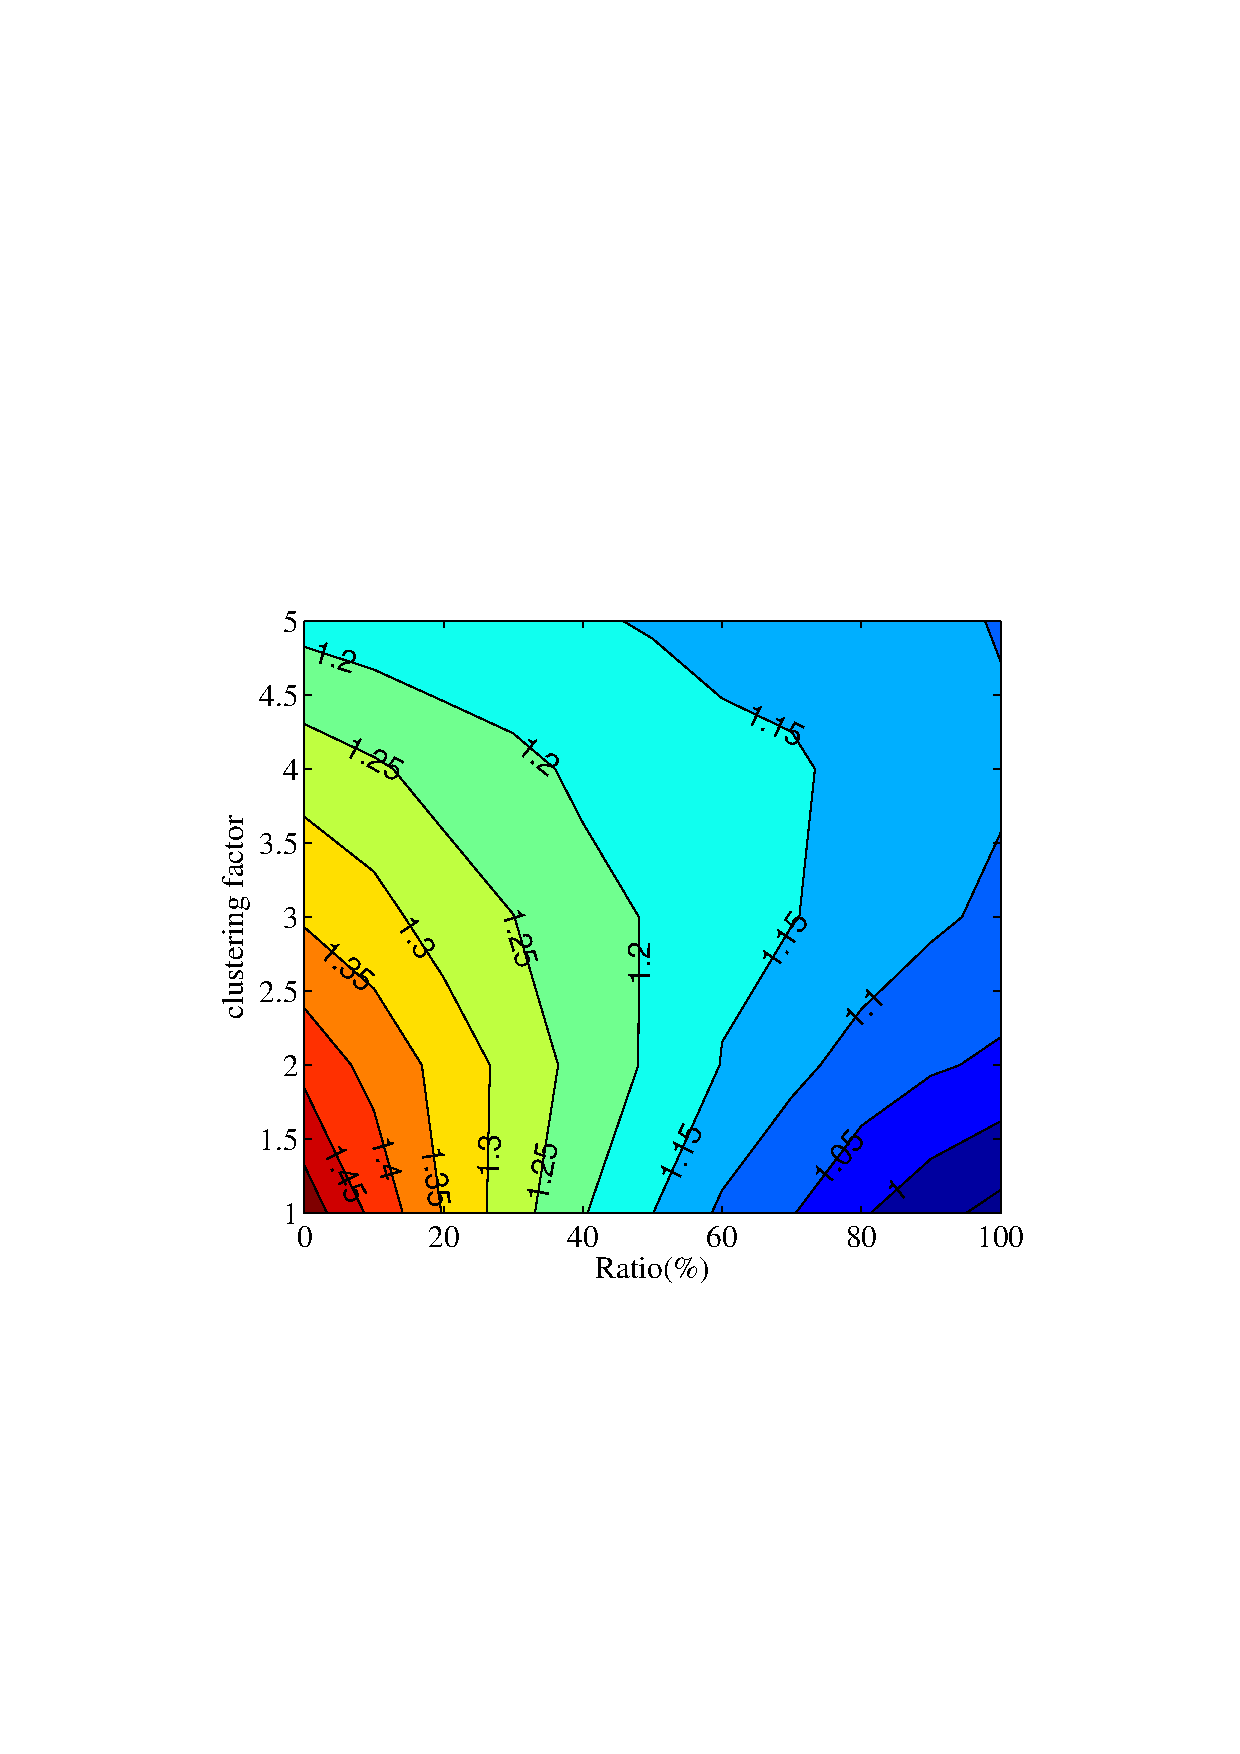
\includegraphics[width=0.8\linewidth]{figure/cfactor.pdf}
	\caption{Experiment 1: Speedup of Horizontal Clustering (HC).}
	\label{fig:shc}
	\vspace{-10pt}
\end{figure}

Experiment 2: Fig.~\ref{fig:performance} (top) shows the performance gain over HC $\mu$ of the balancing methods compared to the HC method for the LIGO workflow. HIFB and HDB significantly increase the performance of the workflow execution. Both strategies capture the structural and runtime information, reducing data transfers between tasks, while HRB focuses on runtime distribution, which in this case is none. Fig.~\ref{fig:performance} (bottom) shows the performance of the balancing methods for the Epigenomics workflow. When increasing the average data size, only HDB demonstrates significantly improvement related to HC. Investigating the structure of the Epigenomics workflow (Fig.~\ref{fig:shape}-bottom), we can see that all tasks at the same horizontal level share the same IFs ($HIFV$ = 0), because each branch (surrounded by dash lines) happen to have the same amount of pipelines. Thus, HIFB has no performance improvement when compared to HC. However, for LIGO (Fig.~\ref{fig:shape}-top), $HIFV \neq 0$, thus HIFB improves the workflow runtime performance.  
%The intuition behind this difference between HDB and HIFB is that 
HDB captures the strong connections between tasks (data dependencies) and HIFB captures the weak connections (similarity in terms of structure). In both workflows, $HDV$ is not zero thus HDB performs better than HC. 

% It is clear that with the increase of the average data size, both HDB and HIFB perform better than HRB. The reason is that both HDB and HIFB can capture the structural information and runtime information, while HRB only focuses on runtime distribution but in this case there is no runtime variance at the horizontal level. 

\begin{figure}[htb]
	\centering
	\includegraphics[width=\linewidth]{figure/exp2_ligo.pdf}
	\includegraphics[width=\linewidth]{figure/exp2_genome.pdf}
	\caption{Experiment 2: Performance of the LIGO workflow (top) and the Epigenomics workflow (bottom).}
	\label{fig:performance}
	\vspace{-10pt}
\end{figure}

Experiment 3: Fig.~\ref{fig:incluence_of_hrv} shows the performance gain $\mu$ when varying task runtimes for the LIGO workflow. As expected, when $HRV$ increases HRB over performs HC. However, HDB and HIFB demonstrate poor performance because they merge tasks based on data dependencies first, and then, they balance the runtime distribution. 
For high values of $HRV$, we just simply need to use HRB. Otherwise, we can use either HDB or HIFB while in some cases HIFB fails to capture the structural information. 

\begin{figure}[htb]
\centering
	\includegraphics[width=\linewidth]{figure/exp3.pdf}
	\caption{Experiment 3: Influence of $HRV$ (LIGO workflow).}
	\label{fig:incluence_of_hrv}
	\vspace{-10pt}
\end{figure}




\input{sensitivity.tex}

\section{Conclusion, Discussion and Future Work}

In this work, we introduced a series of quantitative and structural metrics in revealing workflow structure information and we further applied them to three usage scenario to show their influence with traced based analysis and simulations. The experiments show that these metrics can significantly improve the performance of task clustering strategies and task scheduling strategies.   

In our work, we have shown that these metrics have strong connection with the performance of different optimization methods. However, not all of them perform well under all of the circumstances. Also, the origin of these metrics are heavily depending on human intuition. Still, there is a lack of understanding of whether we can have more and better metrics in revealing how workflow structures interact with different optimization methods. As an initial effort, we will continue to use pattern discovery techniques to collect as many metrics as possible and performance experiments on them. 

With enough metrics, one important step we are going to take is to aggregate multiple metrics and use machine learning techniques to reveal their correlation. However, combining the metrics we have proposed above is challenging. First, these metrics are quantitative and can be measured, however, on their own they are hard to compare against each other and determine whether one metric is more significant than others. Second,  having multiple metrics together increase the complexity and this is against our initial goal, which is reduce the complexity in analyzing workflows. A more sophisticated alternative, however, is to conduct a statistical analysis based on Principal Component Analysis (PCA). This method determines in a more precise way the existing correlation between the collected metrics and their impact on workflow performance.

%A more sophisticated alternative, however, is to conduct a statistical analysis based on Principal Component Analysis (PCA). This method determines in a more precise way the existing correlation between the collected metrics and their impact on resilience. However, undertaking an automated analysis using PCA requires prior experimental data to be available. For this reason, in or- der to better enable a comparison, the aggregation of all the metrics into a single value is proposed in this section. Aggregations of multiple variables are used in many well- known disciplines such as statistical or economic measure- ment. However, combining the metrics we have proposed above provides three main challenges. First, the metrics are quantitative and can be measured, however on their own they are hard to compare against each other and to deter- mine whether one metric is more significant than another. Second, having multiple metrics makes any comparison difficult. Third, resilience increases in direct proportion to some metrics, whereas it reduces with respect to others. Identify- ing to what degree each measured metric impacts resilience (directly or inversely) must also be qualified through previously recorded experimental data or by an expert.

%% References with bibTeX database:

\bibliographystyle{elsarticle-num}
\bibliography{biblio}

%% Authors are advised to submit their bibtex database files. They are
%% requested to list a bibtex style file in the manuscript if they do
%% not want to use elsarticle-num.bst.

%% References without bibTeX database:

% \begin{thebibliography}{00}

%% \bibitem must have the following form:
%%   \bibitem{key}...
%%

% \bibitem{}

% \end{thebibliography}


\end{document}

%%
%% End of file `elsarticle-template-num.tex'.
